\section{Measurement-driven reverse engineering}
\label{sec:measurement}

\subsection{The campaign}

The measurements were taken on four cluster nodes, each with one ConnectX-5 Ex
adapter at 100\,GbE running RoCEv2 with a port maximum transmission unit of
4096, attached over PCIe Gen4 to a single-socket server, all four behind one
leaf switch. Priority flow control is disabled on all eight priorities;
802.3x global pause is enabled at the adapters and, as \S\ref{sec:meas:fabric}
shows, terminates at the switch; DCQCN runs at the firmware default because the
in-tree driver exposes no configuration for it. Two firmware revisions are
present across the four nodes, which turned out to matter
(\anom{09}).

The campaign ran in six phases. Every phase froze an \emph{expectations} file
before its first measurement, naming each claim, the sweep that would test it,
and the numeric band that would count as a match. A claim that missed was
recorded as a miss with its mechanism, and no expectation was edited after the
run. This is what makes several of the results below usable: the most valuable
findings in the campaign are misses, and a miss is only evidence if the
prediction was written down first.

\begin{table}[t]
  \centering
  \small
  \caption{Campaign phases. Records are named as they appear in the campaign
    report tree.}
  \label{tab:phases}
  \begin{tabular}{@{}llr@{}}
    \toprule
    Phase & Record and subject & Points \\
    \midrule
    P1  & \texttt{RESULTS-p1-harness}: instrument hardening, & $\sim$100 \\
        & host-loopback per-type ceilings, PCIe pressure & \\
    P2  & \texttt{RESULTS-p2-msgsize}: message size versus & 291 \\
        & throughput, latency floor, socket comparison & \\
    P3  & \texttt{RESULTS-p3-collie}: anomaly hunt on the wire & 92 \\
    P4  & \texttt{RESULTS-p4-kernels}: replay of serving-kernel & 77 \\
        & burst patterns, gap sweep, skew, duplex & \\
    P5a & \texttt{RESULTS-p5a-incast}: true two-to-one incast & 33 \\
    P5b & \texttt{RESULTS-p5b-tos0}: Not-ECT control and & 48 \\
        & the on-wire type-of-service probe & \\
    P6  & \texttt{RESULTS-p6-fabric}: fabric calibration by & 76 \\
        & endpoint probing, edge-case probes & \\
    \midrule
    & Total & $>$700 \\
    \bottomrule
  \end{tabular}
\end{table}

Two further records carry the analysis rather than the runs.
\texttt{VALIDITY-lossy-fabric} is a validity review, written after P5a, that
marks for each test whether a fabric without priority flow control can support
it at all; it disqualifies the loss-counter channel as standalone evidence near
saturation and restricts the anomaly hunt to the throughput channel.
\texttt{FINDINGS-cx5} is the consolidated ledger: discrepancies between what
was registered and what is true (section~A), issues that bite in practice
(section~B), physics that graduates into the model (section~C), and the fabric
constants (section~D).

\subsection{Evidence classes}

Every parameter that leaves the campaign carries one of five classes, defined
in the project's calibration contract:

\begin{description}\itemsep2pt
  \item[\evdoc{}] defined in a public specification, driver interface or vendor
    manual; the model reproduces the named field, its units, its access and its
    documented semantics.
  \item[\evdrv{}] the behaviour follows from reviewed \texttt{mlx5} or
    \texttt{rdma-core} source but has no public silicon contract; the model
    implements the software-visible behaviour and retains source provenance.
  \item[\evcal{}] the internal stage is not public, but its aggregate effect is
    identifiable from controlled measurement; the model carries a named latent
    parameter with bounds and does not expose a fabricated register.
  \item[\evdecl{}] the value was derived by scaling or by assumption rather than
    measured; every ConnectX-7 field that differs from ConnectX-5 is of this
    class.
  \item[\evinf{}] the value is bracketed by endpoint observations of something
    that is not directly observable, such as a switch buffer measured only
    through its victims.
\end{description}

\subsection{Instruments}

\textbf{perftest}~\cite{perftest} supplied the message-size and latency
sweeps of P2. Its
limitations were found the hard way and are reported below: its bidirectional
mode under-reports, and its single-queue-pair saturation number is a property
of the fabric rather than of the adapter.

\textbf{A patched anomaly-search engine.} P3 through P5b used the traffic
engine from Collie~\cite{collie2022} with seven upstream defects repaired and
one semantic trap disarmed. The trap is worth naming because it invalidates any
unpatched wire experiment: the engine's default local acknowledgement timeout
is the encoding that means \emph{infinite}, so on a fabric that drops, the first
lost packet stalls a reliable requester permanently and silently, at zero rate
and with no error. Every wire point in this campaign ran with a finite timeout.
We further extended the engine with burst pacing (a burst of $N$ message
completions followed by a programmed inter-burst gap) so that P4 could replay
serving-kernel traffic shapes rather than saturating streams.

\textbf{A per-packet ECN and timestamp logger.} P6 required knowing whether a
packet arrived CE-marked, which no counter on this platform reports
truthfully. The logger receives on unreliable-datagram queue pairs with a deep
receive queue, reads the real inbound IP header (which the driver delivers in
the global-routing-header area for RoCEv2 over IPv4), and stamps arrivals with
the adapter's hardware clock. It processed on the order of $10^{8}$ packets per
phase.

\textbf{Counter sampling.} A sampler read the full \texttt{ethtool} and
\texttt{sysfs} counter sets on every participating node at 4\,Hz for
throughput phases and at 100\,Hz where a transient was being timed, with full
before-and-after snapshots bracketing each point. The hardware counters are
cached by the driver for 10\,ms, so rates are computed only over windows of at
least that length.

\subsection{The fixed-offset law and queue-depth dominance}
\label{sec:meas:law}

At a queue depth of one, goodput as a function of message size $S$ follows a
fixed-offset law,
\begin{equation}
  B(S) \;=\; \frac{S}{T_{\text{eff}} + S/C},
  \label{eq:fixedoffset}
\end{equation}
with an effective per-message initiation cost $T_{\text{eff}}$ and an
asymptotic rate $C$. The campaign fitted it twice. P2 fitted
$T_{\text{eff}} = 4.02$\uS{} with $C = 80.6$\Gbps{} over 23 sizes, 22 of them
within 15\,\%. P4, after discovering that the tool flag believed to set queue
depth actually sets the number of work requests per posting call, ran a true
depth-one arm and refitted: $T_{\text{eff}} = 4.48$\uS{} and
$C = 97.1$\Gbps{}, residuals at most 5.1\,\%. The second pair is canonical,
because the first fit's asymptote is the lossy equilibrium of a pipelined loop
rather than a device property. The model half-rate size follows as
$S_{1/2} = T_{\text{eff}} \cdot C \approx 54$\,KiB. For comparison, the
simulator this work feeds had been carrying $8.3$\uS{}.

Queue depth then dominates message size. Figure~\ref{fig:msgsize} plots both
arms. At 8\,KiB a queue that is 1024 deep runs at 77.2\Gbps{} where a queue of
depth one runs at 13.2\Gbps{}, a factor of 5.9; at 512\,KiB the two arms have
converged. Posting batch, by contrast, is nearly free: batches of 1 and 64
differ by $1.16\times$, because both pipeline at the same queue depth. Any
model that predicts a collective from message size alone is therefore wrong by
up to a factor of six in exactly the regime that serving traffic occupies.

\begin{figure}[t]
  \centering
  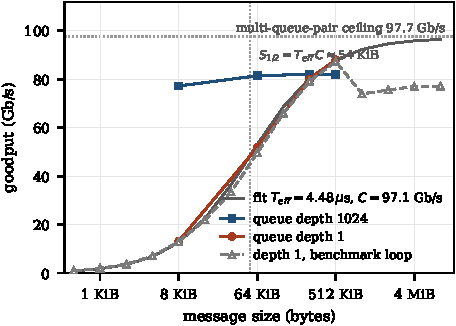
\includegraphics[width=\columnwidth]{figures/msgsize.pdf}
  \caption{Goodput against message size at queue depth 1 and queue depth 1024,
    with Equation~\ref{eq:fixedoffset} fitted to the depth-1 points
    ($T_{\text{eff}} = 4.48$\uS{}, $C = 97.1$\Gbps{}). The depth-1024 arm sits
    on the loss equilibrium of \anom{03} rather than on the ceiling. Data:
    \texttt{RESULTS-p2-msgsize}, \texttt{RESULTS-p4-kernels}.}
  \Description{Log-linear plot of goodput against message size for three arms: a benchmark depth-one loop, a true depth-one engine arm, and a depth-1024 engine arm, with the fixed-offset law fitted to the depth-one points.}
  \label{fig:msgsize}
\end{figure}

The latency floor is 2.10\uS{} median and 2.23\uS{} at the 99th percentile for
a two-byte RDMA write, and 3.99\uS{} for a read, against a measured switch
path of 2.08\uS{}. Against a default TCP socket on the same wire, RDMA is
about $3.5\times$ the bandwidth and about $18\times$ better in latency.

\subsection{The loss equilibrium and the drain window}
\label{sec:meas:drain}

P2 reported a single-queue-pair write and send ``cap'' near 78\Gbps{} that a
second queue pair recovered to the fabric ceiling of 97.7\Gbps{}, and read it
as a requester-side hardware limit. P3 found the number was not constant: send
at 64\,KiB reproduced 78.0\Gbps{} exactly, write at 64\,KiB reached
91.7\Gbps{}, read at 1\,MiB reached 96.7\Gbps{}. P4 resolved it. A single
queue pair sustains 92 to 97\Gbps{} \emph{in burst} at every size. What P2
measured is an equilibrium: a saturated deep pipeline pushes the responder past
its ingress discard threshold, the responder drops at its physical-layer
ingress with no transport signal, and go-back-N recovery costs up to about
16\,\% of goodput. The counter signature is exact and repeatable: the sender
accumulates \ctr{packet\_seq\_err} and \ctr{roce\_adp\_retrans}, the receiver
accumulates \ctr{rx\_discards\_phy}, \ctr{out\_of\_sequence} and a few pause
frames, and \ctr{rx\_out\_of\_buffer} never moves. Depth-one flows and paced
flows are completely clean.

The pacing result is the surprising one. Figure~\ref{fig:drain} shows the gap
sweep. At 8\,KiB, inserting a 4\uS{} inter-burst gap \emph{raises} wall goodput
from 77.5 to 88.2\Gbps{}, a gain of 13.8\,\%, because the gap lets the
responder's ingress drain and removes the retransmission tail entirely. Above
the threshold the duty-cycle model, bytes divided by burst plus gap, is exact
to $\pm 0.1\,\%$; below it, it misses by about 16\,\% at exactly and only the
points where the loss counters move. The threshold is size dependent: at least
4\uS{} at 8\,KiB, and between 4 and 100\uS{} at 64\,KiB, where the 4\uS{}
point still discards about 30\,000 packets per run. Serving decode traffic,
whose per-layer compute gaps run from 4 to 368\uS{}, therefore sits in the
lossless, exactly predictable regime; only back-to-back saturation is lossy.

\begin{figure}[t]
  \centering
  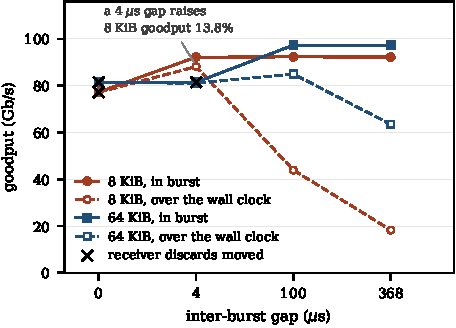
\includegraphics[width=\columnwidth]{figures/drain.pdf}
  \caption{Drain window. Goodput inside a burst and over the wall clock against
    inter-burst gap, at 8\,KiB and 64\,KiB. Points where the receiver's
    \ctr{rx\_discards\_phy} moved are marked. Above the size-dependent
    threshold the duty-cycle model is exact; at 8\,KiB a 4\uS{} gap raises
    wall goodput by 13.8\,\%. Data: \texttt{RESULTS-p4-kernels}.}
  \Description{Line plot of goodput inside a burst and over the wall clock against the inter-burst gap at 8 KiB and 64 KiB, with the points at which the receiver ingress discard counter moved marked.}
  \label{fig:drain}
\end{figure}

Two further asymmetries fall out of the same mechanism. Full duplex is
\emph{cleaner} than one direction: at 91.8\Gbps{} per direction no counter
moves, while a single direction at 93.4\Gbps{} drops, so the responder's
discard threshold sits between the two. And the full-duplex aggregate is
195.0\Gbps{}, which is 99.8\,\% of twice the 97.7\Gbps{} ceiling, with zero
counter movement, at up to 320 queue pairs per direction. The 180\Gbps{} that
P2 reported for the same configuration is an artifact of the benchmark's
bidirectional mode.

\subsection{The internal budget}

Driving loopback traffic and wire traffic into one adapter at once caps total
ingress near 197\Gbps{}, and the split is not fair: the wire flow keeps 99 to
99.8\,\% of its solo rate and the loopback flow absorbs the entire shortfall,
falling to about 51\,\%. The registered hypothesis had been PCIe pressure, and
it is wrong: \ctr{outbound\_pci\_stalled\_rd} and
\ctr{outbound\_pci\_stalled\_wr} were exactly zero at every point of the entire
campaign, including 195\Gbps{} of host-loopback traffic at 4\,MiB across 64
queue pairs. PCIe Gen4 is never the bottleneck at 100\,GbE. What binds is an
internal processing budget with a fixed priority order, and colocated ranks
exchanging over adapter loopback starve under wire load.

\subsection{Congestion control that nobody configured}
\label{sec:meas:cc}

This is the finding the campaign revised most often, and the sequence is worth
stating because the final answer contradicts both the site's belief and our own
two intermediate inferences.

P2 concluded that the fabric never marks ECN, on the evidence that
\ctr{np\_ecn\_marked\_roce\_packets} was zero across 2.5\,TB and $1.09 \times
10^{9}$ packets. P3 corrected that: the same runs moved \ctr{np\_cnp\_sent} and
\ctr{rp\_cnp\_handled} in nearly every phase, so DCQCN was plainly active and
the marking counter is simply inert on these firmware revisions
(\anom{07}). Since a notification point emits a CNP only on receipt of a
CE-marked packet, we inferred that the switch marks. P5a and an endpoint
configuration audit repeated that inference with more evidence: under a
two-to-one incast the receiver emitted 78\,058 CNPs and the senders handled
179\,746, with \ctr{rp\_cnp\_ignored} exactly zero, which proves both a
notification point and a reacting reaction point at firmware default.

P6 refuted the inference at its root. With per-packet logging of $6.7 \times
10^{8}$ packets, at two distinct differentiated-services classes, with the
switch's egress buffer full and dropping 6.36\,\% of traffic, and with 100\,\%
of arriving packets carrying ECT(0) and therefore markable, the number of
CE-marked packets observed was \emph{zero}. The switch does not mark. It
tail-drops, and $K_{\min}$, $K_{\max}$ and $P_{\max}$ are undefined for it.
What generates the notifications is the receiving adapter, from its own ingress
congestion: the receiver's \ctr{np\_cnp\_sent} rises from 38 per second at
idle to 2262 per second exactly during reliable fan-in, which is 283 CNPs per
second per congested queue pair, or one per 3.54\mS{} (\anom{16}). The site's
belief that ECN was off was right about the switch and wrong about the
consequence; our own two intermediate readings were wrong about the marking
point.

A separate probe explains why the traffic was markable in the first place.
P5b requested a Not-ECT control by setting the type-of-service byte to zero and
found the treatment never reached the wire. A standalone probe that reads the
real inbound IP header shows that the adapter overwrites the two ECN bits to
ECT(0) on every RoCEv2 transmit while honouring the differentiated-services
field exactly (\anom{06}):

\begin{center}\small
\begin{tabular}{@{}llll@{}}
  \toprule
  requested & meaning & on the wire & \\
  \midrule
  105 & DSCP 26 $+$ ECT(1)   & 106 & DSCP 26 $+$ ECT(0) \\
  104 & DSCP 26 $+$ Not-ECT  & 106 & DSCP 26 $+$ ECT(0) \\
  0   & DSCP 0 $+$ Not-ECT   & 2   & DSCP 0 $+$ ECT(0) \\
  2   & DSCP 0 $+$ ECT(0)    & 2   & unchanged \\
  \bottomrule
\end{tabular}
\end{center}

Not-ECT RoCE cannot be produced from verbs on this adapter. The practical
consequence is that a default collective job, which sets no type of service at
all, is exactly as ECN-capable and as DCQCN-controlled as our instrumented
traffic, so the congestion behaviour measured here is a property of the
deployment rather than of the harness.

The reaction dynamics are slow. Under a two-to-one incast the first rate cut of
at least 30\,\% arrives after 3, 16 and 39\mS{} in three repeats, fair share is
reached after 5\mS{}, 1.8\,s and 2.3\,s, and recovery to at least 95\,\% of the
solo rate takes $447 \pm 10$\mS{}. The increase is additive at about 0.107
falling to 0.093\Gbps{} per millisecond. The steady two-flow split is 50.18 and
50.13\Gbps{} on a 99.30\Gbps{} wire. Compared with the algorithm's published
defaults the reaction is 2 to 20 times slower and the recovery about
$4.5\times$ slower (\anom{18}), so any study that needs the transient must
carry these numbers and not the defaults.

\subsection{Incast is a tax, not a collapse}

Two senders into one receiver at 1\,MiB messages fill the wire, 99.39\Gbps{}
received, and deliver 73.89\Gbps{} of application goodput. The missing
26.9\,\% of the link is retransmission. The fabric drops 1.65\,\% of packets,
and because each loss forces go-back-N recovery, that 1.65\,\% amplifies about
$16\times$ into the goodput deficit (\anom{11}). Two independent accountings,
the receiver's \ctr{rx\_write\_requests} counter multiplied by message size and
the senders' own completion accounting, agree to 0.02\,\%. The identity is
\begin{equation}
  B_{\text{app}} \;=\; B_{\text{wire}} \cdot
    \bigl(1 - p_{\text{loss}} \cdot A_{\text{gbn}}\bigr),
  \label{eq:incasttax}
\end{equation}
with DCQCN holding $p_{\text{loss}}$ near $10^{-3}$ and $A_{\text{gbn}}$ the
go-back-N amplification factor, measured at about 16 here. That number is worth
a second look: the whole message is 256 packets at this maximum transmission
unit, so retransmitting an entire message on every loss would give
$A_{\text{gbn}} = 256$ and a goodput of zero. The measured 16 says the unit
that is actually replayed is the requester's outstanding window, about 64\,KiB,
and not the message. $A_{\text{gbn}}$ is therefore \evcal{}: it is bounded above
by $S_{\text{msg}}/S_{\text{pkt}}$, it grows with message size, and its value
is a property of a window whose size the specification does not fix.

Fair share is excellent, 50.4 against 49.6, with a four-hertz standard deviation of 0.26\Gbps{} and no
starvation. Fan-out is free: one sender to two receivers delivers 97.83\Gbps{}
split 50.000 to 50.000 with zero counter movement. Only fan-in pays.

At small messages there is no incast penalty at all. A single sender reaches
16.7 million 512-byte messages per second, and the two-sender aggregate reaches
20.5 million, which is 23\,\% \emph{above} the best single sender: at that size
the system is bound by the sender's message rate, not by the receiver or the
wire. Unreliable datagrams under the same two-to-one overload deliver exactly
$0.500 \pm 0.000$ of the offered load with zero movement on every watched
counter at all three nodes (\anom{12}), which is the lossy fabric in one
number.

\subsection{The fabric under the endpoint}
\label{sec:meas:fabric}

P6 calibrated the fabric from the endpoints, because no switch counters were
available. The four nodes share one non-blocking leaf: the latency matrix over
all six pairs spans 1.98 to 2.11\uS{}, a range of 0.13\uS{}, which is smaller
than the repeat-to-repeat spread within one direction and far below the
0.6 to 2.0\uS{} that one extra hop would add; sixteen fresh five-tuples are
unimodal within 0.10\uS{}, so there is one path and no measurable equal-cost
multipath from these nodes; a ring of four runs at 391.94\Gbps{} with every
port at 97.98\Gbps{}.

The per-port egress buffer is a tail-drop queue of about 5.2\,MB.
Figure~\ref{fig:incast} (bottom) shows the identity that measures it: two paced senders
step from below to above the port rate, and the product of the excess rate and
the time from the start of queue build to the first sustained loss is constant
at 5.04 to 5.39\,MB across excess rates of 4.8, 9.7 and 19.7\Gbps{}, a spread
of 6.8\,\%. An independent estimate from the post-overload drain tail gives
$5.76 \pm 2.45$\,MB. The drain rate is 99.995\Gbps{} in all twelve runs, and
loss in steady overflow equals the excess rate to better than 0.04\Gbps{}.
The buffer is \evinf{}: it is measured entirely through its victims.

\begin{figure}[t]
  \centering
  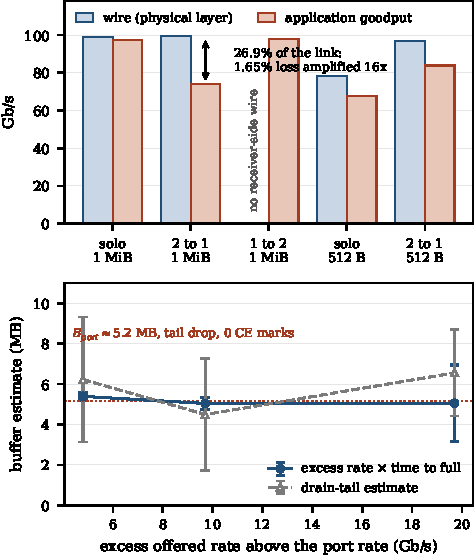
\includegraphics[width=\columnwidth]{figures/incast.pdf}
  \caption{Top: the incast tax. Physical-layer receive rate against
    application goodput for the two-to-one cases and their solo and fan-out
    controls. The wire stays full and the deficit is retransmission. Bottom:
    the switch buffer identity. Excess rate times time to buffer-full is
    constant across three excess rates, giving a tail-drop egress buffer of
    about 5.2\,MB; the independent drain-tail estimate is shown beside it, and
    the fraction of packets marked congestion-experienced is zero at every
    point. Data: \texttt{RESULTS-p5a-incast}, \texttt{RESULTS-p6-fabric}.}
  \Description{Two stacked panels. The top panel is a grouped bar chart of physical-layer wire rate against application goodput for five incast and control cases. The bottom panel plots two independent switch buffer estimates against the excess offered rate.}
  \label{fig:incast}
\end{figure}

There is no link-level flow control anywhere in the path. Priority flow control
is off in the hardware register on every node; the adapters do emit 802.3x
global pause under load, on the order of 760 frames per run, and
\ctr{rx\_pause\_ctrl\_phy} is zero at every node in every phase of the entire
campaign. The pause loop is one hop long, receiver to switch, and terminates
there (\anom{08}).

Finally, a lone reliable flow above about 94\Gbps{} loses $0.1798\,\% \pm
0.0012$ of its packets at the receiver's physical-layer ingress, over eight
repeats and 32 fresh five-tuples, unimodal and path independent. The loss is
bursty: about 73 packets, roughly 94\uS{}, per event. At least 10\Gbps{} of
reverse traffic cuts the event count by $12.5\times$ without changing the burst
length, 1\Gbps{} of reverse traffic does nothing, and receiver CPU load does
nothing. \ctr{rx\_out\_of\_buffer} is zero in every run, so this is not receive
queue exhaustion. This is \anom{17}, and no block in the model reproduces its
mechanism yet.

\subsection{Counters do not mean what they say}

Any tool that detects RDMA anomalies from counters has to know four things
about this hardware (\anom{19}, \anom{09}, \anom{07}).
\ctr{packet\_seq\_err} counts loss \emph{bursts}, not lost packets: under a
lone flow the receiver discarded 107\,542 packets while the sender recorded
1\,465 sequence errors, a ratio of about 73, because go-back-N collapses one
contiguous drop burst into one sequence error. \ctr{rx\_discards\_phy} counts
adapter-ingress loss exactly, and switch-side loss appears in neither counter.
\ctr{rx\_out\_of\_buffer} never moves, in any phase, because receive queues
were always posted deep and RDMA writes consume none. \ctr{rx\_write\_requests}
is an exact application-goodput counter, agreeing with engine accounting to
0.01\,\%, but it is 32 bits wide and wraps at high message rates.
\ctr{np\_ecn\_marked\_roce\_packets} is inert. Firmware 16.31 counts
\ctr{local\_ack\_timeout\_err} where firmware 16.32 counts zero for identical
behaviour. And senders handle $2.24\times$ the CNPs the receiver reports
sending, reproducibly, which we record and do not explain.

\subsection{Corrected attributions}

Three widely quoted numbers from this campaign are wrong as originally
attributed, and the corrections are part of the result.

The 78\Gbps{} single-queue-pair ``cap'' is a loss and retransmission
equilibrium of a saturated deep pipeline on a fabric without flow control, not
a requester limit; in burst the same queue pair reaches 92 to 97\Gbps{}.

The 3.07 million packets per second single-queue-pair unreliable-datagram
receive cap, along with a spectacular 47.5\,\% silent discard, belonged to the
measurement engine's receive path and not to the adapter. On the wire, with the
per-packet logger instead of the engine, one receive queue pair absorbs 5.51
million 2\,KiB packets per second and 2.98 million 4\,KiB packets per second
with only the 0.17 to 0.19\,\% ingress floor, and four queue pairs are slightly
worse. The row survives in the anomaly table with kind \textit{tool}
(\anom{01}), reproduced by nothing, because deleting it would erase the reason
several downstream numbers changed.

The 129\Gbps{} unreliable-datagram ceiling measured on host loopback is
packets-per-second bound and does not transfer: on the wire the same transport
is bandwidth bound and clean at 99.4\Gbps{}.

\subsection{The anomaly table}

Table~\ref{tab:anomaly} is the campaign's output in the form the architecture
consumes. Each row names a trigger, an effect with a magnitude, an evidence
phase, and a \emph{kind} that says how the model is required to reproduce it:
\textit{emergent} from a named mechanism and validated against a band,
\textit{injected} by rule because the mechanism is not public,
\textit{fabric} because it belongs to the switch or the link, \textit{counter}
because it is a facade behaviour with no datapath effect, or \textit{tool}
because it is an artifact of the instrument. The table is data, not prose: it
is a constant array in the model's sources with a generated projection that a
test compares byte for byte, and one test per row asserts the effect inside its
registered band.

\begin{table*}[t]
  \centering
  \footnotesize
  \setlength{\tabcolsep}{3.5pt}
  \renewcommand{\arraystretch}{1.12}
  \caption{The nineteen-row anomaly table: the verification contract between
    the measurements and the architecture. \textit{Kind} states how the model
    is required to reproduce the row. The block column names the block of
    \S\ref{sec:arch} that owns it. Rows \anom{01} and \anom{16} through
    \anom{19} are post-specified corrections made after the phase that owns
    them was frozen, and are labelled as such in the campaign records.}
  \label{tab:anomaly}
  \newcolumntype{R}[1]{>{\raggedright\arraybackslash}p{#1\textwidth}}
  \begin{tabular}{@{}l R{0.115} R{0.185} R{0.30} R{0.065} l l@{}}
    \toprule
    Id & Anomaly & Trigger & Effect and magnitude & Kind & Block & Evidence \\
    \midrule

    \anom{01} & UD receive cap &
    one UD queue pair receiving above 3.07\,Mpps through the measurement engine &
    re-attributed: the knee and the 47.5\,\% silent loss were the engine's
    receive path. On the wire one UD queue pair absorbs 5.51\,Mpps of 2\,KiB
    with only the 0.17 to 0.19\,\% ingress floor &
    tool & none & P3, P6 \\

    \anom{02} & two-SGE send sequence-error storm &
    RC send with two gather entries of 512\,B each, 32 queue pairs &
    \ctr{packet\_seq\_err} of 68\,k to 400\,k per 30\,s; the one-entry control
    at identical bytes is exactly zero; goodput within 3\,\% &
    injected & B7, B8 & P3 \\

    \anom{03} & saturated loss equilibrium &
    one RC queue pair, queue depth 1024, no inter-burst gap, above about
    92\Gbps{} &
    responder ingress discards plus a go-back-N tail; goodput settles at 78 to
    92\Gbps{} &
    emergent & B10 & P2, P3, P4 \\

    \anom{04} & drain window &
    inter-burst gap of at least 4\uS{} at 8\,KiB, 4 to 100\uS{} at 64\,KiB &
    discards go to zero; goodput follows the duty model within 0.1\,\%; a
    4\uS{} gap raises 8\,KiB goodput by 13.8\,\% &
    emergent & B10 & P4 \\

    \anom{05} & loopback starvation &
    loopback and wire ingress together above 197\Gbps{} &
    wire keeps 99\,\%, loopback drops to 51\,\%, no PCIe stall &
    emergent & B17 & P3 \\

    \anom{06} & ECT(0) stamping &
    any RoCEv2 transmit &
    ECN bits forced to ECT(0) regardless of requested type of service; DSCP
    honoured &
    injected & B7 & P5b \\

    \anom{07} & inert marking counter &
    any traffic &
    \ctr{np\_ecn\_marked\_roce\_packets} stays zero while CNPs are generated &
    counter & B19 & P3, P5a, P5b \\

    \anom{08} & one-hop pause &
    receiver overload &
    receiver emits global pause; no peer ever receives one &
    fabric & B9 $+$ fabric & P3, audit \\

    \anom{09} & firmware counter variant &
    retransmission &
    firmware 16.31 counts \ctr{local\_ack\_timeout\_err}; firmware 16.32
    counts zero &
    counter & B19 & P5a \\

    \anom{10} & duplex cleaner than simplex &
    full duplex at 91.8\Gbps{} per direction against one direction at
    93.4\Gbps{} &
    duplex counter-clean, simplex dirty; the discard threshold sits between &
    emergent & B10 & P4 \\

    \anom{11} & incast amplification &
    $N$ senders into one receiver, 1\,MiB messages &
    wire full; goodput tax equals loss rate times a go-back-N amplification
    factor ($16\times$ at 1.65\,\% loss, a 26.9\,\% tax) &
    emergent & B7, B13 & P5a \\

    \anom{12} & UD one-over-$N$ delivery &
    $N$ UD senders into one receiver &
    delivery exactly $1/N$; no endpoint counter moves &
    fabric & fabric & P5a \\

    \anom{13} & MTU tax &
    path MTU 1024 against 4096 &
    5.6\,\% of goodput &
    emergent & B7 & P2 \\

    \anom{14} & host-bound message rate &
    small messages, single process &
    3.87\,Mpps on one queue pair at 1\,KiB; 16.7\,Mmsg/s per sender at 512\,B &
    emergent & B6 & P2, P5a \\

    \anom{15} & memory-region insensitivity &
    12\,000 memory regions; 1024 regions of 64\,KiB; gathers except \anom{02} &
    no throughput effect &
    emergent by absence & B5 & P3 \\

    \anom{16} & endpoint-generated notification &
    RC fan-in on a fabric whose switch never marks &
    the receiver signals its own ingress congestion: \ctr{np\_cnp\_sent} rises
    from 38 to 2262 per second, which is 283 CNP/s per congested queue pair &
    emergent & B14 & P6 \\

    \anom{17} & ingress stall bursts &
    one lone RC flow above about 94\Gbps{} &
    0.18\,\% of packets lost at the receiver's ingress in bursts of about 73
    packets (94\uS{}), path independent over 32 five-tuples; 10\Gbps{} of
    reverse traffic cuts the event count $12.5\times$ without changing the
    burst length &
    emergent & B10 & P6 \\

    \anom{18} & slow DCQCN dynamics &
    a reaction point under two-to-one RC fan-in &
    cut of at least 30\,\% after 3 to 39\mS{}; fair share after 5\mS{} to
    2.3\,s; recovery to 95\,\% in $447 \pm 10$\mS{}; additive increase about
    0.1\Gbps{} per millisecond &
    emergent & B15 & P6 \\

    \anom{19} & counter semantics under loss &
    any loss on the path &
    \ctr{packet\_seq\_err} counts loss bursts, $73\times$ fewer than packets
    lost; \ctr{rx\_discards\_phy} is exact; switch loss appears in neither;
    \ctr{out\_of\_buffer} never moves; senders handle $2.24\times$ the CNPs the
    receiver reports sending &
    counter & B19 & P6 \\

    \bottomrule
  \end{tabular}
\end{table*}

